\documentclass[12pt]{report}

\newcommand{\langname}{Funguwuage}
\newcommand{\lang}{\texttt{\langname} }

\title  {\langname\ Developer's Manual}
\author {Rylan Lens Kellogg}

\newlength{\inprogramwidth}
\settowidth{\inprogramwidth}{A few lines of text in a block.}

% Easy, interactive cross-references with '\hyperref[label]{text}'.
\usepackage[hidelinks]{hyperref}
% Prevent section titles from appearing at the bottom of pages!
\usepackage[nobottomtitles, nobottomtitles*]{titlesec}
% Fancy verbatim markup, for better source code.
\usepackage{fancyvrb}
% Fancy headers, for chapter title page headers
\usepackage{fancyhdr}
% Easy flow charts and other simple diagrams
\usepackage{smartdiagram}
% Very complicated diagram drawing
\usepackage{tikz}
\usetikzlibrary{arrows, shapes}

% For tables
\usepackage{tabularx, array, multirow}

% For programs
\usepackage{listings}

% I don't want to deal with putting \ after ‘i.e.’ etc., and also
% double spacing isn't really that common anymore nowadays...
%
% Note: most confusingly, the command ‘\frenchspacing’ turns French
% spacing off (!).
\frenchspacing

\newcommand\ie{i.\,e.}
\newcommand\eg{e.\,g.}

% Math mode columns
\newcolumntype{C}{>{$}c<{$}}

% Footnotes should be flushed left with no indent.
\makeatletter
\renewcommand\@makefntext[1]{%
	\setlength\parindent{1em}%
	\noindent
	\llap{\textsuperscript{\@thefnmark}\kern.5pt}{#1}%
}
\makeatother

% \titleformat{<command>}[<shape>]
% {<format>}
% {<label>}
% {<sep>}
% {<before-code>}
% {<after-code>}

% Remove numbering from chapter heading.
%\titleformat  {\chapter} [hang]
%{ \normalfont\huge\bfseries }
%{}{ 0pt }
%{  }
%{  }
% Make chapter heading snug up to top of page.
\titlespacing*{\chapter}{-21pt}{-72pt}{10pt}

% Remove numbering from section heading.
%\titleformat  {\section} [hang]
%{ \normalfont\Large\bfseries }
%{}{ 0pt }
%{  }
%{  }
% Make section heading have a sensible amount of spacing around it.
\titlespacing*{\section}{-10pt}{24pt}{10pt}

% Set variable paragraph skip (vertical blank space between paragraphs).
\setlength{\parskip}{3pt plus 3pt minus 1pt}


% I should probably just use geometry, but this works so...

% Move fancy header upwards. It's like halfway down the page by default.
\setlength{\headheight}{14.5pt}
\addtolength{\topmargin}{-64pt}
% Extend text downwards, it stops with like 3 inches on the bottom.
\addtolength{\textheight}{128pt}

% Smart diagram style(s)
\smartdiagramset{
  monotone/.style={
    uniform arrow color   = true,
    arrow color           = black,
    uniform color list    = white!60 for 20 items,
    back arrow disabled   = true
  }
}

\begin{document}

% I have no idea how this works but it puts the chapter name at the top of each page.
% https://stackoverflow.com/a/48735234
\pagestyle{fancy}
\renewcommand{\chaptermark}[1]{\markboth{#1}{#1}}
\fancyhf{}
\fancyhead[C]{\leftmark}
\fancyfoot[C]{\thepage}

% Title Page
\hypersetup{pageanchor=false}
\begin{titlepage}
  \maketitle
\end{titlepage}

\tableofcontents

\chapter{Overview}
\label{ch:Overview}

Currently, \lang has three stages (or phases, or levels, anything to that regard; we'll call them stages).

\begin{center}
  \smartdiagramset{
    monotone,
    text width = 4cm,
    module x sep = 5cm,
    font = \large
  }
  \smartdiagram[flow diagram:horizontal]{
    Parsing,
    Type-checking,
    Code Generation
  }
\end{center}

The parser converts \lang source code into a data structure that represents the program in it's entirety.

The type-checker then validates this data structure, ensuring that the semantics of types are being followed properly.

The code generation stage creates a new data structure (an in-memory intermediate representation) that follows static single assignment form.
This intermediate representation gets converted by each backend into
architecture specific implementations (machine code, asm, etc).

\chapter{Parsing}
\label{ch:parsing}

The parsing stage validates and begins to understand the syntax of \lang source code.

The parsing stage can be thought of as two systems that work together: the \emph{lexer} and the \emph{parser}. The parser drives the parsing stage, and calls to the lexer as needed.

The parser keeps track of all state (how much has been parsed so far, etc). The lexer is a simple tool to increment the state of the parser. The parsing state state consists of a lexeme, it's length in bytes, and a pointer to the end of the lexeme (where we will begin lexing from next). This pointer starts at the beginning of our source code, and makes it's way towards the end as the parser advances the parsing state.

\section{Lexer}
\label{subsec:lexer}

The lexer's job is to split up the input source code into understandable chunks (called lexemes); after all, the file is read as one, large, arbitrary sequence of bytes. The lexer splits these bytes into understandable pieces, and also strips off parts of the file that aren't needed, like whitespace and comments.

The lexer must not lex more than one lexeme at a time. It is the job of the parser to understand sequences of lexemes.

\vspace{1em}

There are two main actions the lexer can make:
\begin{itemize}
\item[advance] Get the lexeme directly after the given position, updating position to end of new lexeme.
\item[expect]  Get the lexeme directly after the given position, only updating position if the given lexeme was found.
\end{itemize}

\begin{minipage}{\textwidth}

Given the following source code:
\begin{Verbatim}[samepage=true]
  ;; Intercept Simple Lexing Example
  a : integer
  a := 69
\end{Verbatim}

The lexer would produce the following lexemes (line separated) from the above source code, on subsequent calls.
\begin{Verbatim}[samepage=true]
  a
  :
  integer
  a
  :
  =
  69
\end{Verbatim}
\end{minipage}

\section{Parser}
\label{subsec:parser}

The parser is the main component of the parsing stage, and does most of the heavy lifting.

The job of the parser is to create an understanding of the program, from the compiler's point of view. To do this, the program must be unambigous, and contain only sequences of lexemes that are understood.

One thing you may be wondering: how does a computer program (the compiler) \emph{know} something? How can you make it \emph{understand}? The idea is that by defining a data structure in our compiler that can store the meaning of programs, as well as any necessary data along with it, the compiler can construct one of these structures and end up with an understood program, because the data structure is already understood.

There are two usual choices for data structures that can fully define the semantics of a program, while also storing data along with it.

One, the most common, is called an \emph{abstract syntax tree}, or AST. The AST is a fancy name for a tree that houses only the bare minimum data of what is needed for the program moving forward. For example, parentheses aren't needed in an AST, because they don't actually do anything. They are only for the parser to understand what order to parse things in; since we don't need them after that (the AST is already constructed in the right order), they don't get included in the AST itself. This is why it is an \emph{abstract} syntax tree; the tree doesn't map one-to-one with the source code syntax. Some compilers do build what's called a parse tree that does map one-to-one with the source code.

Another, still fairly common, is called a \emph{directed acyclic graph}, or DAG. A DAG is much like an AST, except that it is not a tree structure, but a graph. This means any node can be connected to any node, and lots of complicated group and category theory ensues. Because a single node can be referenced by any other node, it does mean that it takes less memory to store the same program, and is likely more efficient overall. The problem lies within it's complexity: DAGs are hard to manage, and when it goes wrong, it goes very, very wrong. However, it is clear that a DAG is better in almost every way than an AST, if you are willing to deal with the headaches.

For the sake of simplicity and understanding, \lang uses an AST, or abstract syntax tree, and generates it from recognized sequences of lexemes.

A tree, in computer programming, is a data structure that can branch into multiple data structures. An AST happens to be a recursive tree, in that each of the branches of the tree can have branches, and those branches can have branches, and so on. A lot of compilers use a binary tree, or btree, which is a tree with a recursive left hand side and right hand side. The problem you see in using binary trees is that it is rather difficult to represent anything with more than two children (as one might expect). This is quite a common case in programming language ASTs; for example, when calling a function, there may be any amount of arguments. Most compilers go the LISP route, and have these sort of lists implemented as recursive pairs, where as long as the lhs is another pair, the list continues. I feel like this is a messy implementation, and results in code that is quite hard to read, due to chains of dereferences, \ie{} \verb|lhs->lhs->rhs->value|.

The compiler includes a text-debug format to print the abstract syntax tree that is produced, and can be printed out for any program by adding the verbose command line flag: \verb|-v|.
% NOTE: It would be cool to output this printout into a file and have our own little file format to save this intermediate step. This would help a load if we wanted to start doing conditional compilation.

\begin{minipage}{\textwidth}

Let's take a look at an example. Given the following source code:
\begin{Verbatim}[samepage=true]
  ;; Intercept Parsing Example
  fact : integer (n : integer) = integer (n : integer) {
    if n < 2 {
      1
    } else {
      n * fact(n - 1)
    }
  }

  fact(5)
\end{Verbatim}

The parser would produce the following abstract syntax tree:
\begin{Verbatim}
  PROGRAM
    VARIABLE DECLARATION
      SYM:"fact"          <- colon separates node type from node value
    VARIABLE REASSIGNMENT
      SYM:"fact"
      FUNCTION
        SYM:"integer" (0) <- refers to level of pointer indirection
        NONE              <- empty node to store list of parameter types
          SYM:"integer"
        NONE              <- empty node to store list of body expressions
          IF
            BINARY OPERATOR:"<"
              VARIABLE ACCESS:"n"
              INT:2
            NONE          <- stores 'then' body
              INT:1
            NONE          <- stores 'otherwise' body
              BINARY OPERATOR:"*"
                VARIABLE ACCESS:"n"
                FUNCTION CALL
                  SYM:"fact"
                  BINARY OPERATOR:"-"
                    VARIABLE ACCESS:"n"
                    INT:1
    FUNCTION CALL
      SYM:"fact"
      INT:5
\end{Verbatim}

As you can see, this is a complete representation of the program. It is able to understand high level concepts that the programmer construed in the source code, like conditional control flow, variable accesses, function calls with arguments, and more.

\end{minipage}


\chapter{Type-checking}
\label{ch:typechecking}

Type-checking refers to the process of ensuring the types of expressions are what they are expected to be.

This is only relevant due to \lang being statically typed. This means the type of a variable is known at compile-time, due to the programmer declaring it. This declared type is associated with the variable, and any expressions assigned to it must return a compatible type. It also comes into play with binary expressions: they operate on two objects, each of some type. It wouldn't make any sense to try to add a function to an array, would it? Function calls' arguments must match a function's declared parameters' types. A dereference may only operate on a pointer. All of these semantics of the language are enforced by the type-checker.

\chapter{Code Generation}
\label{ch:codegen}

Finally, we arrive at code generation. This is definitely the most complicated part, and is where compiler developers get lost for decades. While \lang started as a very simple, x86\_64-only compiler, it is slowly growing to become a compiler that supports many backends, each of which cross platform themselves.

Thanks to Sirraide, our compiler has an intermediate representation. I didn't budge easy, but he was insistent and convincing.

If you are like me, you may wonder why this IR is even needed; it seems (at least to me) like it is of no use, and everything it represents could be stored in the AST. If you are not like me, that's good. You're probably smart :P.

Here is a list of reasons that were used to convince myself of using an IR:
- There are none.

Seriously, you can do everything with just an AST, I promise. If you don't want an IR, don't use one. In the early versions of the compiler (that I wrote), there was no IR and codegen happened straight from AST. It wasn't always optimal but through peephole optimizations I'm fairly sure we could get it very good. In any case, Sirraide insisted and made the PR, and I won't turn down a chance to learn something I don't know.

First of all, in the intermediate representation, that doesn't conform to any hardware standard, there are some assumptions that can be made. If there are no hardware limitations, then every value could just be stored in a new register; why wouldn't there be infinite? With this, we would never have to worry about slow-downs from RAM access or an appalling disk IO situation: it would simply always be register to register movement, and only when the user dereferences something would we begin to have memory accesses generated. It's like a code optimizers wet dream: everything in a register, and only explicit memory accesses.

% END INTRO

\begin{Verbatim}[samepage = true]
  ;; Intercept Intermediate Representation Example
  ;; Expressions are annotated with numbers for easy referencing.

  ;; Let us assume that input_condition and if_condition are somehow
  ;; different every time the program runs, like parameters.
  input_condition : integer           ; 0
  if_condition : integer              ; 1

  a : integer                         ; 2
  b : integer = 420                   ; 3
  c : integer = 69                    ; 4
  d : integer                         ; 5
  e : integer                         ; 6
  f : integer                         ; 7

  while 1 {                           ; 8, 9

    a := b + c                        ; 10
    d := a * -1                       ; 11
    e := d + f                        ; 12

    if input_condition {              ; 13, 14
      f := 2 * e                      ; 15
    } else {
      b := d + e                      ; 16
      e := e - 1                      ; 17
    }

    b := f + c                        ; 18
  }
\end{Verbatim}

And the generated AST of the program:
\begin{Verbatim}
  PROGRAM
    VARIABLE DECLARATION:"input_condition"    ; 0
    VARIABLE DECLARATION:"if_condition"       ; 1
    VARIABLE DECLARATION:"a"                  ; 2
    VARIABLE DECLARATION:"b"                  ; 3
    VARIABLE ASSIGNMENT
      SYM:"b"
      INT:420
    VARIABLE DECLARATION:"c"                  ; 4
    VARIABLE ASSIGNMENT
      SYM:"c"
      INT:69
    VARIABLE DECLARATION:"d"                  ; 5
    VARIABLE DECLARATION:"e"                  ; 6
    VARIABLE DECLARATION:"f"                  ; 7
    WHILE                                     ; 8
      INT:1                                   ; 9
      NONE
        VARIABLE ASSIGNMENT                   ; 10
          SYM:"a"
          BINARY OPERATOR:"+"
            VARIABLE ACCESS:"b"
            VARIABLE ACCESS:"c"
        VARIABLE ASSIGNMENT                   ; 11
          SYM:"d"
          BINARY OPERATOR:"*"
            VARIABLE ACCESS:"a"
            INT:-1
        VARIABLE ASSIGNMENT                   ; 12
          SYM:"e"
          BINARY OPERATOR:"+"
            VARIABLE ACCESS:"d"
            VARIABLE ACCESS:"f"
        IF                                    ; 13
          VARIABLE ACCESS:"input_condition"   ; 14
          NONE
            VARIABLE ASSIGNMENT               ; 15
              SYM:"f"
              BINARY OPERATOR:"*"
                INT:2
                VARIABLE ACCESS:"e"
          NONE
            VARIABLE ASSIGNMENT               ; 16
              SYM:"b"
              BINARY OPERATOR:"+"
                VARIABLE ACCESS:"d"
                VARIABLE ACCESS:"e"
            VARIABLE ASSIGNMENT               ; 17
              SYM:"e"
              BINARY OPERATOR:"-"
                VARIABLE ACCESS:"e"
                INT:1
        VARIABLE ASSIGNMENT                   ; 18
          SYM:"b"
          BINARY OPERATOR:"+"
            VARIABLE ACCESS:"f"
            VARIABLE ACCESS:"c"
\end{Verbatim}

Previously, this AST would be used to generate code by the code generation backend (the frontend delegates to different backends based on defaults or configuration at the command line). However, this now gets converted into the following IR (excluding initial variable declarations, only for the sake of brevity in the initial basic block):

Here is the while loop body from our current program, in terms of \lang's intermediate representation, or IR.
\begin{center}
  \begin{tikzpicture}[
    > = latex', auto,
    block/.style = {
      rectangle,
      draw=black,
      thick,
      align=flush center,
      rounded corners,
      minimum height=4em
    },]
\matrix [column sep=5mm,row sep=7mm]{
  % row 1
  &
  \node [block, text width=\inprogramwidth] (firstbox) {
    a := b + c    ; 10

    d := a * -1    ; 11

    e := d + f    ; 12
  }; & \\
  % row 2
  & \node[block] (if) {
    if input\_condition ; 13, 14
  }; & \\
  \node [block] (b1) {
    f := 2 * e    ; 15

  }; &
  & \node [block] (b2) {
    b := d + e    ; 16
    \\
    e := e - 1    ; 17
  };\\
  & \node [block] (d1) {
    b := f + c    ; 18
  };\\
};

\draw[->] (firstbox) -- (if);
\draw[->] (if) -| (b1);
\draw[->] (if) -| (b2);
\draw[->] (b1) -v (d1);
\draw[->] (b2) -v (d1);
% Arrow with label
% \draw[->] (b2) -v (d1) node[midway,above left] {-10};

\draw[-latex,black] ($(d1.east) + (.4,0)$) arc
    [
        start angle = 90,
        end angle =   -80,
        x radius =    6cm,
        y radius =    -3.6cm
    ] ;
\end{tikzpicture}
\end{center}

Each box with code within it is referred to as a \emph{basic block}. \\
The diagram above illustrates the basic blocks of the "main" \emph{function} in our example program and their relation to one another.

\begin{itemize}
\item[Basic Block]
  A flat list of IR instructions that must end in a branch.
\item[Function]
  A flat list of basic blocks with at least an entry and a return block specified, although they may be the same.
\end{itemize}

However, this diagram does not actually conform to \lang's intermediate representation; there is one more step to complete before it matches one-to-one: conversion into static single assignment form, or SSA form for short.

\section{Static Single Assignment Form}
\label{sec:codegen-ssa}

A variable has different values at different times throughout the program, all with different lifetimes... They almost sound like different variables! Wait... what if they were?

Each assignment of a variable after the first creating a new variable is the entire idea behind \emph{SSA}, or static single assignment, form. SSA form is a form of program in which each variable does not get assigned more than one time.

Let's take a look at the example above, converted into SSA form.
\begin{center}
  \begin{tikzpicture}[
    > = latex', auto,
    block/.style = {
      rectangle,
      draw=black,
      thick,
      align=flush center,
      rounded corners,
      minimum height=4em
    },]
\matrix [column sep=5mm,row sep=7mm]{
  % row 1
  &
  \node [block, label = above:{\small bb0}, text width=\inprogramwidth] (firstbox) {
    $a_1$ := b + c    ; 10

    $d_1$ := $a_1$ * -1    ; 11

    $e_1$ := $d_1$ + f    ; 12
  }; & \\
  % row 2
  & \node[block, label = below:{\small bb1}] (if) {
    if input\_condition ; 13, 14
  }; & \\
  \node [block, label = left:{\small bb2}] (b1) {
    f := 2 * $e_1$    ; 15

  }; &
  & \node [block, label = left:{\small bb3}] (b2) {
    $b_1$ := $d_1$ + $e_1$    ; 16
    \\
    $e_2$ := $e_1$ - 1    ; 17
  };\\
  & \node [block, label = above:{\small bb4}] (d1) {
    $b_2$ := f + c    ; 18
  };\\
};

\draw[->] (firstbox) -- (if);
\draw[->] (if) -| (b1);
\draw[->] (if) -| (b2);
\draw[->] (b1) -v (d1);
\draw[->] (b2) -v (d1);
% Arrow with label
% \draw[->] (b2) -v (d1) node[midway,above left] {-10};

\draw[-latex,black] ($(d1.east) + (.4,0)$) arc
    [
        start angle = 90,
        end angle =   -81,
        x radius =    6.8cm,
        y radius =    -4.18cm
    ] ;
\end{tikzpicture}
\end{center}

% TODO: They are up above, but maybe should be here? Basic block, function, value, etc. vocabulary definitions...

The above diagram is not what the actual data structure appears as, so let's take a look at a lower level representation of the intermediate representation. How about that?

\begin{itemize}
\item[\%]
  A temporary value, like a register on a CPU.
\item[bb]
  A basic block within a function.
\item[fun]
  A function with a list of basic blocks.
\end{itemize}


\begin{Verbatim}[samepage = true]
fun main:
  bb0:
    %r0 = global_load("b")
    %r1 = global_load("c")
    %r2 = add(%r0, %r1)
    global_store(%r2, "a") ;;  10
    %r3 = global_load("a")
    %r4 = immediate(-1)
    %r5 = multiply(%r3, %r4)
    global_store(%r5, "d") ;; 11
    ;; ...
\end{Verbatim}

% TODO: There has to be a better title than this!
\section{Variable Liveness}
\label{sec:codegen-variable-liveness}

WARNING: The following section contains vocabulary regarding topics of life and death, due to this being what it has been called in many, many learning resources. We hope to move away from these possibly offensive terms, and towards something we can all discuss without bad memories being brought up.

\begin{itemize}
\item[Live]
  A temporary is considered live after it has been assigned and up until the last use of this temporary.
\item[Live Range]
  The range of expressions in a basic block in which a temporary is live.
\end{itemize}

Liveness analysis is done by keeping track of every use of some calculated value in a linked list of \verb|Use| structures (pronounce like the noun, the 'S' is voiceless). This is done during intermediate representation generation. Effectively, we build our IR with live ranges built-in.

If a temporary is live during the definition of another temporary, the two temporaries are said to \emph{interfere}.

Excerpt from demonstration IR above:
\begin{Verbatim}
  %r0 = global_load("b")   ;; a
  %r1 = global_load("c")   ;; b
  %r2 = add(%r0, %r1)      ;; c
  global_store(%r2, "a")   ;; d
  %r3 = global_load("a")   ;; e
  %r4 = immediate(-1)      ;; f
  %r5 = multiply(%r3, %r4) ;; g
  global_store(%r5, "d")   ;; h
\end{Verbatim}

Live ranges from above excerpt:
\begin{Verbatim}
    r0 r1 r2 r3 r4 r5
  a |
  b |  |
  c |  |  |
  d       |
  e          |
  f          |  |
  g          |  |  |
  h                |
\end{Verbatim}

\chapter{Register Allocation}
\label{sec:codegen-register-allocation}
An IR function may contain a potentially infinite number of temporaries; a physical CPU, by contrast, has only a limited number
of \textit{physical} or \textit{hardware registers}. Register allocation (RA) is the process of assigning to each temporary a register
in such a way that no two interfering temporaries share a register. This is accomplished mainly by means of an \textit{interference graph}.

The interference graph of an IR function is an undirected graph consisting of a set of vertices and a set of edges between those
vertices; every temporary in the function is represented by a vertex, and an edge is drawn between each pair of temporaries that
interfere. The problem of finding an (ideal) allocation of at most $k$ registers to those temporaries is then equivalent to the problem
of finding an (ideal) $k$-colouring of the interference graph.

The process of $k$-colouring a graph $G$ consisting of vertices $V$ and edges $E$ consists in assigning to each vertex $v \in V$ a colour
from $1$ to $k$, such that no vertex $v'$ with $vv' \in E$ (that is, no vertex $v'$ adjacent to $v$) has that same colour.

Or, to put it differently: the process of assigning at most $k$ registers to the temporaries that make up  a function consists in assigning
 to each temporary a register between $1$ and $k$ such that no temporary that interferes with it is assigned that same register.

Unfortunately, graph colouring—and by extension register allocation—cannot be solved in polynomial time in the general
case,\footnote{The colouring part of register allocation for a program in SSA form \textit{is} possible in polynomial time; however, if we
also include PHI lowering and everything else that goes into register allocation, the RA process overall is still NP-complete.} unless
P = NP, which is one reason why this entire process ends up being as complicated as it is.

The following sections are only a high level overview of RA; both the actual implementation and the theory behind it are rather complex,
and writing a register allocator that can account for every last quirk that an architecture may have and which can correctly allocate
registers for any well-formed IR program is a fairly complicated endeavour, and our current register allocator is still a far cry from that.

Nevertheless, in what follows, we present a hopefully not too complicated description of the general RA process, as well as the theory
and ideas behind it, the reasons as to why certain things are implemented the way they are, and finally, the shortcomings of the current
implementation.

\section{PHI Elimination}
The first step of our register allocation algorithm concerns \textit{PHI ($\Phi$) instructions}. Of all the instructions in our IR, the PHI
instruction is easily the most difficult to grasp, as it is a rather abstract concept that is found in all SSA languages, and yet, there
are no physical CPUs that implement anything like it.

As the name might suggest, the central concept of an SSA language like our IR is exactly that: \textit{single static assignment}. Once
created, a temporary can \textit{never} be reassigned, and its value is guaranteed to be the same throughout the entire function. This
works just fine in most cases: most instructions only consume and produce values, but never alter them; even variable reassignment,
can be expressed as a sequence of load and store instruction without any actual reassignment.

Where it leads to problems is in situations where control flow demands that different values be used depending on what path is taken,
and while it may theoretically be possible to solve this by employing a temporary store/load to/from memory, we would much rather keep
temporaries in registers for as long as possible and only evict them to memory once we start running out of registers.

The classical example of such a situation is the following \langname{} program (declarations are omitted for the sake of brevity):
\begin{Verbatim}
a := if b {
  ;; Code that computes ‘c’
  c
} else {
  ;; Code that computes ‘d’
  d
}
\end{Verbatim}

\noindent Compiling this program to IR yields:
\begin{Verbatim}
bb1:
    %b = ... ;; Code that computes ‘%b’
    branch on %b to bb2 else bb3
bb2:
    %c = ... ;; Code that computes ‘%c’
    branch to bb4
bb3:
    %d = ... ;; Code that computes ‘%d’
    branch to bb4
bb4:
    %a = phi [bb1: %c], [bb2: %d]
\end{Verbatim}

\noindent The PHI instruction \verb|%a = phi [bb1: %c], [bb2: %d]| means ‘assign to \verb|%a| the value of \verb|%c| if we reached this block
from \verb|bb1|, and the value of \verb|%d| if we reached this block from \verb|bb2|’; this way, we can assign different values to \verb|%a|
depending on the control flow of the program, without having to assign to \verb|%a| twice.

It is important to realise that a PHI instruction is a very high-level construct. The LLVM documentation quite aptly refers to it as ‘the
magical mystical PHI node, that can not exist in nature, but can be synthesized in a computer scientist's overactive imagination’. The PHI
instruction here merely tells us \textit{what} values must be assigned to \verb|%a|—it does not contain or provide us with any information
whatsoever as to \textit{how} this should be accomplished.

Thus, before we can even begin to talk about register allocation proper, we must first convert these PHIs into something that can
actually be assigned a register, or several registers. This process is referred to as \textit{PHI lowering} or \textit{PHI elimination}
both here and in the source code of the RA, but it is also often known by other names such as \textit{PHI lifting} or \textit{SSA
destruction}.

Lowering PHIs seems simple at first glance: simply insert a copy from \verb|%c| in \verb|bb2| and from \verb|%d| in \verb|bb3| to
\verb|%a| before the branch to \verb|bb4|;\footnote{Note that copying to an SSA temporary, thereby changing its value, breaks the
aforementioned SSA invariant; as a result of this, the program will no longer be in SSA form after PHI lowering, hence the term ‘SSA
destruction’.} no code is ultimately generated at the actual location of the PHI itself, but we
still allocate a register for it, and that is the register that we copy \verb|%c| or \verb|%d| into. After register allocation, we may
end up with something like this:
\begin{Verbatim}
bb1:
    %r1 = ... ;; Code that computes ‘%r1’ (%b)
    branch on %r1 to bb2 else bb3
bb2:
    %r2 = ... ;; Code that computes ‘%r2’ (%c)
    %r4 = copy %r2
    branch to bb4
bb3:
    %r3 = ... ;; Code that computes ‘%r3’ (%d)
    %r4 = copy %r3
    branch to bb4
bb4:
    ;; In this case, the RA has assigned %r4 to %a.
    ;;
    ;; No code is generated for the PHI; the copy
    ;; instructions that we inserted above have
    ;; already placed the right value into %r4 by
    ;; the time we get to this point in the program.
\end{Verbatim}

\noindent Depending on the complexity of the program, a good register allocator may even be able to generate the values of \verb|%b| and
\verb|%c| directly in \verb|%r4|, which would make the copies unnecessary since the values would already be in the right register.

Unfortunately for us, this strategy of simply inserting copies everywhere does not always work. There are two big problems with this
approach, one of which is rather easy to solve (and the solution is implemented in our RA), the other one\ldots{} not so much.

\subsection{Critical Edges}
The first problem occurs when an argument of a PHI instruction originates in a block that has a \textit{critical edge}. A critical edge is
defined as an edge between a block with multiple successors and a block with multiple predecessors (though in our case, it only matters
that the block has multiple successors).

Consider the following IR program:
\begin{Verbatim}
bb1:
    %b = ...
    %c = ...
    branch on %b to bb2 else bb4
bb2:
    %d = ...
    %e = ...
    branch on %e to bb3 else bb4
bb3:
    ;; Some lengthy computation
    ;; ...
    return
bb4:
    %a = phi [bb1: %c], [bb2: %d]
\end{Verbatim}

\noindent Trying to lower the PHI in \verb|bb4| by simply inserting copies in the blocks above doesn't quite work in this case:
\begin{Verbatim}
bb1:
    %r1 = ...
    %r2 = ...
    %r4 = copy %r2
    branch on %r1 to bb2 else bb4
bb2:
    %r3 = ...
    %r5 = ...
    %r4 = copy %r3
    branch on %r5 to bb3 else bb4 (*)
bb3:
    ;; Some lengthy computation
    ;; ...
    return
bb4:
    ;; Value of ‘%a’ is supposed to be in %r4 here.
\end{Verbatim}

\noindent At first glance, it might seem as though there were nothing wrong with this program; and indeed, it works just fine, so long
as the \verb|(*)| branch instruction always branches to \verb|bb4|. However, what happens if control flow branches to \verb|bb3| instead?
In that case, we still end up copying \verb|%r3| to \verb|%r4|—even if its value isn't used in \verb|bb3|! This means that \verb|%r4|
cannot be used at all in \verb|bb3|!

As to why that is the case, consider the following scenario: assume there is some value \verb|%v| that is computed somewhere before
\verb|bb2| and which is used in \verb|bb3|, but not in \verb|bb4| or any of its successors. Assume futher that we (incorrectly) allow
the use of \verb|%r4| in \verb|bb3|; in this case, the RA may decide to assign \verb|%r4| to both \verb|%v| and \verb|%a|. If we consider
only the semantics of our original IR pre PHI lowering, then this assignment is perfectly reasonable: \verb|%v| is only used up to
\verb|bb3|, and unused in \verb|bb4| and after, and \verb|%a| is only used in \verb|bb4| and after. The liveness ranges of \verb|%v| and
\verb|%a| do not overlap, and therefore, they may be assigned the same register.

However, during PHI lowering, we end up inserting a copy instruction from \verb|%r3| to \verb|%r4| in \verb|bb2|. This means that the value
of \verb|%v|, which was held in \verb|%r4| up to this point, is overwritten with \verb|%r3|, \textit{irrespective of what block we branch
to}. Everything is fine so long as we branch to \verb|bb4|, but if we branch to \verb|bb4|, then we have problem, since \verb|bb4|
expects the value of \verb|%v| to be stored in \verb|%r4|, but we've just overwritten it with the value of \verb|%r3|.

This illustrates that we can't just insert copies into a block that ends with a conditional branch. Fortunately, this problem has a rather
simple solution: if copy insertion is problematic in blocks that contain a conditional branch, then we simply need to insert the copy in a
block that contains only an unconditional branch instead. This can be accomplished by inserting an additional block between \verb|bb2| and
\verb|bb4| and generating the copy instruction in that block:
\begin{Verbatim}
bb1:
    %r1 = ...
    %r2 = ...
    branch on %r1 to bb2 else bb1-copy
bb1-copy:
    %r4 = copy %r2
    branch to bb4
bb2:
    %r3 = ...
    %r5 = ...
    branch on %r5 to bb3 else bb2-copy
bb2-copy
    %r4 = copy %r3
    branch to bb4
bb3:
    ;; Some lengthy computation
    ;; ...
    return
bb4:
    ;; Value of ‘%a’ can now be in %r4.
\end{Verbatim}

\noindent This way, the right values are always in \verb|%r4| by the time control flow reaches \verb|bb4|, but at the same time, \verb|%r4|
is never clobbered if control flow branches to \verb|bb3| instead. We can now safely use \verb|%r4| for both \verb|%v| and \verb|%a| without
changing the semantics of the program.

\subsection{Multiple PHIs in One Block}
The second problem that one might encounter is less intuitive, but it too is a direct result of SSA form. In order to uphold the invariants
of SSA form, all PHIs in a block must execute \textit{simultaneously} and immediately upon entering the block; or at least, they must
behave as such when lowered.

This is best illustrated with an example. Consider the following program:
\begin{Verbatim}
bb1:
    %a1 = ...
    %a2 = ...
    branch to bb3
bb2:
    %b1 = ...
    %b2 = ...
    branch to bb3
bb3:
    %c1 = phi [bb1: %a1], [bb2: %b1]
    %c2 = phi [bb1: %a2], [bb2: %b2]
\end{Verbatim}

\noindent Assuming the latest uses of \verb|%a1| and \verb|%a2|, as well as of \verb|%b1| and \verb|%b2|, are in the PHIs in \verb|bb3|, we
might end up with the following register allocation:
\begin{Verbatim}
bb1:
    %r1 = ... (%a1)
    %r2 = ... (%a2)
    branch to bb3
bb2:
    ;; Yes, %r1 and %r2 are the other way around here
    ;; on purpose; the RA might decide to do this if,
    ;; for example, the value previously stored in %r1
    ;; is required to compute %r2.
    %r2 = ... (%b1)
    %r1 = ... (%b2)
    branch to bb3
bb3:
    %r1 = phi [bb1: %r1], [bb2: %r2]
    %r2 = phi [bb1: %r2], [bb2: %r1]
\end{Verbatim}

\noindent Here, the RA has allocated only two registers for the six temporaries; normally, this would be desired since not only do we waste
fewer registers, but especially in the case of a PHI, it is doubly beneficial for its result and one or more of its arguments to share a
register, seeing as the latter need to be copied into the former either way, and copying from a register to itself is a no-op.

This program, as is, is perfectly fine, but you may notice that we haven't inserted any copies for the PHIs yet. That was done on purpose
to show how this program, which is, again, perfectly correct \textit{while still in SSA form}, breaks as soon as we try to lower the PHIs:
\begin{Verbatim}
bb1:
    %r1 = ... (%a1)
    %r2 = ... (%a2)

    ;; Ok, no-op
    %r1 = copy %r1
    %r2 = copy %r2

    branch to bb3
bb2:
    %r2 = ... (%b1)
    %r1 = ... (%b2)

    ;; ERROR
    %r1 = copy %r2
    %r2 = copy %r1

    branch to bb3
bb3:
    %r1 = phi [bb1: %r1], [bb2: %r2]
    %r2 = phi [bb1: %r2], [bb2: %r1]
\end{Verbatim}

\noindent You may notice that a recurring effect of lowering PHIs seems to be that everything works out just fine—so long as we only ever
follow one control flow path, in this case from \verb|bb1| to \verb|bb3|. However, if we reach \verb|bb3| from \verb|bb2|, then everything
breaks down: unfortunately, \verb|%r1| needs to be copied into \verb|%r2|, but \verb|%r2| needs to be copied into \verb|%1|! In
other words, we need to swap two registers. If we simply try to lower these two PHIs by inserting copies like we have done so far, we end
up overwriting one of the values with the other. This what we mean when we say that SSA expects all PHIs to execute simultaneously.

In some cases, swapping the contents of two registers can be a non-trivial problem that may involve using a third register, which then also
needs to be allocated, or evicting the contents of either register into memory and then loading it back into the other. Alternatively, we
could also just swap the values by performing three \verb|xor|s or by using some sort of \verb|swap| instruction (\verb|xchg| on
x86\textunderscore64), provided the target architecture allows for that.

So what's the deal with this then? Sure, this is a bit annoying, but it seems rather easy to solve: just swap them, right? Well, in this
case, yes, but what if instead of two PHIs, we had to lower three, or ten.\footnote{This may, at first glance, seem like an absurd number of
PHIs, but consider that if we want to optimise local variables by converting them to temporaries, we will eventually have to insert PHIs for
variables that are assigned to in multiple different control flow paths.} At that point, we would be confronted with a complex scheduling
problem since efficient register allocation might lead to certain registers’ being assigned to both the result of a PHI and arguments of
potentially \textit{several} PHIs. Generally speaking, this problem is not that easy to solve, which is why our RA currently does not
permit more than one PHI per block.

\section{Interference Graph}
The next step is to build the interference graph of the function. This interference graph has two representations: an adjacency matrix and
a set of adjacency lists. First, we construct the matrix and perform register coalescing (more about that later), and then we convert the
matrix into a set of adjacency lists; those lists are the input for the actual graph colouring portion of the algorithm.

\subsection{Adjacency Matrix}
The adjacency matrix $M$ is a $n×n$ lower triangular matrix, where $n$ is the number of temporaries that need to be allocated. Each temporary
is assigned an index between $1$ and $n$. Given two temporaries whose indices are $i$ and $j$, the entry $M_{\max(i,j),\,\min(i, j)}$ is $1$ if
those temporaries interfere, and $0$ otherwise.\footnote{Since ‘interferes with’ is a symmetric relation, we only need to store either
$M_{i,j}$ or $M_{j, i}$. Here, we arbitratily choose to always put the larger index first.} The values on the main diagonal are unused since
there is never a reason to check if a temporary interferes with itself.

For example, given a program with 5 temporaries $t_1$–$t_5$ in which $t_1$ interferes with $t_3$, $t_2$ with $t_1$, and $t_3$ with $t_5$, the
adjacency matrix of the interference graph of that program looks as follows:\medskip

\noindent\begin{tabular}{@{}C|CCCCC}
 & t_1& t_2& t_3& t_4& t_5\\\hline
t_1& & & & & \\
t_2&1& & & & \\
t_3&1&0& & & \\
t_4&0&0&0& & \\
t_5&0&0&1&0& \\
\end{tabular}\medskip

\noindent This matrix is constructed by the following algorithm:
\lstset{%
	language=algol,
	basicstyle=\ttfamily,
	keywordstyle=\bfseries,
	emph={%
		TEMPORARY, ADJMATRIX, ADJLIST, RETURN
	}, emphstyle={\bfseries}
}
\begin{lstlisting}
PROC build adjacency matrix = ([] TEMPORARY ts) ADJMATRIX:
BEGIN
    ADJMATRIX m;

    FOR i FROM 1 TO length (ts) DO
        FOR j FROM 1 TO length (ts) DO
            IF interfere (ts[i], ts[j]) THEN
                m[max (i, j), min (i, j)] = 1
            FI
        OD
    OD;

    RETURN m
END
\end{lstlisting}

\noindent The function \verb|interfere (ts[i], ts[j])| returns \verb|TRUE| if the $i$-th and $j$-th temporaries interfere, and \verb|FALSE|
otherwise. It accomplishes this by iterating over all the uses of \verb|ts[i]| and checking if the definition of \verb|ts[j]| lies
between the definition of \verb|ts[i]| and the use, and vice versa.\footnote{Recall that two temporaries interfere iff either one is live
at the definition point of the other, for which reason we only need to search for the definition point of \texttt{ts[j]} within the live
range of \texttt{ts[i]}, and vice versa.} If any of the uses interfere, then the temporaries interfere.

\subsection{Adjacency Lists}
The other representation of the Interference Graph is a set of adjacency lists, one for each vertex (temporary). The adjacency list of a
temporary $t$ contains, amongst other things, the set of temporaries that interfere with $t$, as well as the set of physical registers that
interfere with $t$.\footnote{Whether and what physical registers interfere with a temporary depends on the target architecture, the type of
the instruction that computes the temporary and other temporaries in that instruction, as well as on  physical registers are stored into
or clobbered while the temporary is live.} The former can be computed by looking at the adjacency matrix and the latter by examining the
live range of each temporary.

\section{Coalescing}
After we build the adjacency matrix and before we build the adjacency lists, there is yet another step that is commonly referred to as
\textit{coalescing}. The main purpose of coalescing is copy elision: we try to remove as many copy instructions from the IR as possible.

Consider the copy instruction \verb|%a = copy %b|. If the live range of \verb|%b| ends with that copy instruction, \ie{} if \verb|%b| is not
used afterwards, then we may be able to generate the value of \verb|%b| in \verb|%a| instead, effectively combining (or \textit{coalescing})
\verb|%a| and \verb|%b| into one temporary. We can then remove the copy instruction.

Since our backend makes liberal use of precoloured copy instructions so as to make sure that certain values end up in the right registers
where necessary (\eg{} the actual parameters of a function call),\footnote{Precoloured in this case means that we have already assigned a
physical register to the result of an instruction. For instance, if \texttt{\%a} is the first argument of a function call, then—on Linux—we
will need to make sure that that value ends up in \texttt{\%rdi}, for which reason we insert a \texttt{\%rdi = copy \%a} instruction before
the call.} coalescing can help drastically reduce the number of copy instructions in the generated code.

Coalescing is an iterative process: we iterate over all temporaries, merge copies, and remove copy instructions that are no longer needed
from the IR. This is repeated until no more copy instructions are removed, at which point we also need to rebuild the adjacency matrix
since merging two temporaries entails merging their live ranges: any other temporary that previously interfered with either temporary now
interferes with the merged temporary. Since this can lead to more live ranges overlapping, coaleascing can also have the adverse effect
of increasing the chromatic number\footnote{The \textit{chromatic number} of a graph is the number of colours required to colour the graph,
or, in our case, the total number of registers that need to be allocated for a function.} of the interference graph; our RA currently does
not take this into account.

\section{Colouring}
After lowering PHIs, building the adjacency matrix, coalescing, and building the adjacency lists, we can finally move on to the actual
colouring process. Our register allocator uses the Chaitin-Briggs algorithm. This algorithm is a two-step process\footnote{Strictly
speaking, proper Chaitin-Briggs register allocation also involves a third step: spilling temporaries that cannot be assigned a register.
However, since our programs, at least for the time being, are unlikely to be so complex as to necessitate spilling, the RA currently does
not implement it and simply terminates should it find that the interference graph is not $k$-colourable.} and relies on two
principles.

First, a graph $G$ is $k$-colourable if (\textit{not} iff) for every vertex $v$ in $G$, $\deg(v) < k$.\footnote{$\deg(v)$ denotes the
\textit{degree} of $v$. The degree of a vertex is the number of adjacent vertices, or, in our case, the number of temporaries that
interfere with the temporary associated with the vertex.} Furthermore, given a graph $G$ containing a vertex $v$ with $\deg(v) < k$,
$G$ is $k$-colourable iff $G - v$ is $k$-colourable.\footnote{The proof of these theorems is left to the reader; this is not a textbook
on graph theory, after all.} In simpler terms, this means that every vertex that has fewer than $k$ neighbours
can be coloured, and removing that vertex does not affect the $k$-colourability of the graph.

Thus, the first step of the Chaitin-Briggs algorithm is to iterate over all vertices in the interference graph, removing all vertices
with degree $< k$ and pushing them onto a stack. A removed vertex no longer interferes with any other vertex in the graph (but we still
keep track of what values it used to interfere with; this information is still needed later). This also means that removing a vertex may
cause previously adjacent vertices with degree $\geq k$ to now have degree $< k$, and therefore, those vertices can now be removed as well
and so on. This procedure is repeated until no more vertices are removed. Ideally, the graph should now be empty. If it isn't we move on
to step 2.

Chaitin’s original algorithm would spill\footnote{Spilling a temporary means storing its value into memory, thus freeing up a register, and
loading it back when it is next needed.} a vertex as soon as there are no more vertices with degree $< k$. However, recall that all
vertices having degree $< k$ is only sufficient and not necessary for a graph to be $k$-colourable. Even if a vertex has degree $\geq k$, we
might still be able to $k$-colour the graph. The most famous example of this is the graph below, which is $2$-colourable, but Chaitin’s
algorithm would spill a vertex when trying to $2$-colour it:
\begin{center}
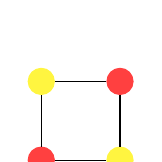
\begin{tikzpicture}
\node[circle, draw, fill, color=red!75]    (A1) at (0,0) {};
\node[circle, draw, fill, color=yellow!75] (B1) at (1,0) {};
\node[circle, draw, fill, color=yellow!75] (C1) at (0,1) {};
\node[circle, draw, fill, color=red!75]    (D1) at (1,1) {};
\draw (A1) -- (B1);
\draw (A1) -- (C1);
\draw (D1) -- (B1);
\draw (D1) -- (C1);
\end{tikzpicture}
\end{center}

\noindent Briggs’ improvement to Chaitin’s algorithm consists in removing a vertex and putting it onto the stack, even if it has degree
$\geq k$, because the graph might still be $k$-colourable. If it isn’t, we‘ll find out later, and then we’ll have to spill.

Once the interference graph is empty, we can pop vertices off the stack one by one and assign to each vertex a register that has not yet
been assigned to any of its neighbours. If there are no registers left that we could assign to a vertex, then this is where we spill the
vertex. As mentioned before, our register allocator currently does not account for that and simply aborts if that happens. But if everything
goes well, we now have a properly register-allocated function!

\section{Example}
This section illustrates step by step how a \langname{} program is compiled from source code to register-allocated IR. We will be compiling
the following program (declarations are once again omitted for the sake of brevity; ‘\ldots’ informally indicates omitted instructions that
ultimately produce a value):
\begin{Verbatim}
e := ...
f := ...
a := b + c;
d := b + if a {
  e
} else {
  f
}
\end{Verbatim}

\noindent First, the program is converted to our SSA IR:
\begin{Verbatim}
bb1:
    %e = ...
    %f = ...
    %a = add %b, %c
    branch on %a to bb2 else bb3
bb2:
    branch to bb4
bb3:
    branch to bb4
bb4:
    %tmp = phi [bb2: %e], [bb3: %f]
    %d   = add %b, %tmp
\end{Verbatim}

\noindent Next, we perform PHI elimination:
\begin{Verbatim}
bb1:
    %e = ...
    %f = ...
    %a = add %b, %c
    branch on %a to bb2 else bb3
bb2:
    %tmp = copy %e
    branch to bb4
bb3:
    %tmp = copy %f
    branch to bb4
bb4:
    %tmp = phi [bb2: %e], [bb3: %f]
    %d   = add %b, %tmp
\end{Verbatim}

\noindent Once that's done, it's time to build the adjacency matrix:\medskip

\noindent\begin{tabular}{@{}c|ccccccc}
        &\tt\%a&\tt\%b&\tt\%c&\tt\%d&\tt\%e&\tt\%f&\tt\%tmp\\\hline
\tt\%a  &      &      &      &      &      &      &        \\
\tt\%b  &1     &      &      &      &      &      &        \\
\tt\%c  &0     &1     &      &      &      &      &        \\
\tt\%d  &0     &0     &0     &      &      &      &        \\
\tt\%e  &1     &1     &1     &0     &      &      &        \\
\tt\%f  &1     &1     &1     &0     &1     &      &        \\
\tt\%tmp&0     &1     &0     &0     &0     &0     &        \\
\end{tabular}\medskip

\noindent Next, we perform coalescing; here, we are able to merge \verb|%e| and \verb|%tmp|:
\begin{Verbatim}
bb1:
    %e = ...
    %f = ...
    %a = add %b, %c
    branch on %a to bb2 else bb3
bb2:
    branch to bb4
bb3:
    %e = copy %f
    branch to bb4
bb4:
    %e = phi [bb2: %e], [bb3: %f]
    %d = add %b, %e
\end{Verbatim}

\noindent We can now rebuild the matrix\footnote{For the sake of brevity, we won't show that step here since its identical to how we
constructed the matrix above, albeit with one fewer temporary.} and build the adjacency lists:
\begin{Verbatim}
%a: [%e, %f]
%b: [%c, %e, %f]
%c: [%b, %e, %f]
%d: []
%e: [%a, %b, %c, %f]
%f: [%a, %b, %c, %e]
\end{Verbatim}

\noindent The interference graph looks like this:
\begin{center}
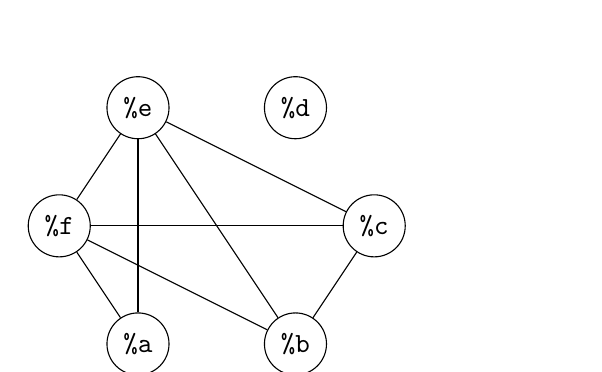
\begin{tikzpicture}

\node[circle, draw] (A) at (0,0)    {\tt \%a};
\node[circle, draw] (B) at (2,0)    {\tt \%b};
\node[circle, draw] (C) at (3,1.5)  {\tt \%c};
\node[circle, draw] (D) at (2,3)    {\tt \%d};
\node[circle, draw] (E) at (0,3)    {\tt \%e};
\node[circle, draw] (F) at (-1,1.5) {\tt \%f};

\draw (B) -- (C);
\draw (B) -- (E);
\draw (B) -- (F);
\draw (C) -- (E);
\draw (C) -- (F);
\draw (E) -- (A);
\draw (F) -- (A);
\draw (F) -- (E);

% Draw an invisible stack so everything lines up.
\node[] (S)  at (5,3.25) {\hphantom{Stack}};
\draw[color=white] (4, 3.5) -- (4, -.5);

\end{tikzpicture}
\end{center}

\noindent This graph is $4$-colourable, so let’s use $4$ registers; we now iterate over all vertices in no particular order and remove all
vertices with degree $<4$. Dashed circles indicate removed vertices and dashed lines indicate removed edges.
\begin{center}
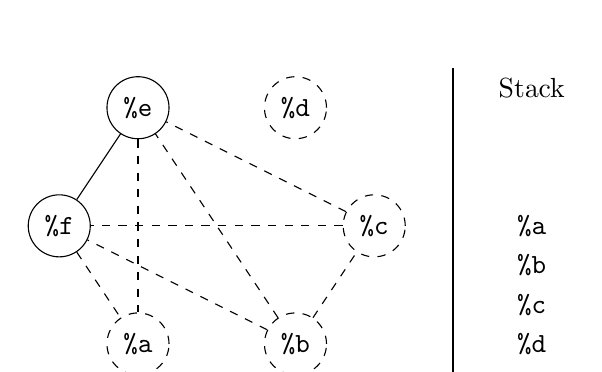
\begin{tikzpicture}
\node[circle, draw, dashed] (A) at (0,0)    {\tt \%a};
\node[circle, draw, dashed] (B) at (2,0)    {\tt \%b};
\node[circle, draw, dashed] (C) at (3,1.5)  {\tt \%c};
\node[circle, draw, dashed] (D) at (2,3)    {\tt \%d};
\node[circle, draw] (E) at (0,3)    {\tt \%e};
\node[circle, draw] (F) at (-1,1.5) {\tt \%f};

\draw[dashed] (B) -- (C);
\draw[dashed] (B) -- (E);
\draw[dashed] (B) -- (F);
\draw[dashed] (C) -- (E);
\draw[dashed] (C) -- (F);
\draw[dashed] (E) -- (A);
\draw[dashed] (F) -- (A);
\draw         (F) -- (E);

\node[] (S)  at (5,3.25) {Stack};
\node[] (S4) at (5,1.5)  {\tt \%a};
\node[] (S3) at (5,1)    {\tt \%b};
\node[] (S2) at (5,.5)   {\tt \%c};
\node[] (S1) at (5,0)    {\tt \%d};

\draw (4, 3.5) -- (4, -.5);
\end{tikzpicture}
\end{center}

\noindent Now, do the same thing again. Note how the vertices \verb|%e| and \verb|%f|, which previously had degree $4$, now have degree $1$:
\begin{center}
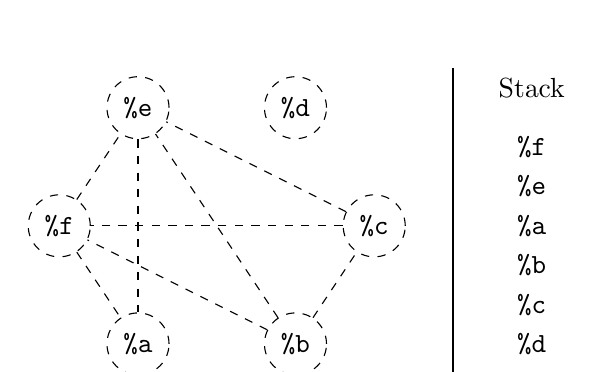
\begin{tikzpicture}
\node[circle, draw, dashed] (A) at (0,0)    {\tt \%a};
\node[circle, draw, dashed] (B) at (2,0)    {\tt \%b};
\node[circle, draw, dashed] (C) at (3,1.5)  {\tt \%c};
\node[circle, draw, dashed] (D) at (2,3)    {\tt \%d};
\node[circle, draw, dashed] (E) at (0,3)    {\tt \%e};
\node[circle, draw, dashed] (F) at (-1,1.5) {\tt \%f};

\draw[dashed] (B) -- (C);
\draw[dashed] (B) -- (E);
\draw[dashed] (B) -- (F);
\draw[dashed] (C) -- (E);
\draw[dashed] (C) -- (F);
\draw[dashed] (E) -- (A);
\draw[dashed] (F) -- (A);
\draw[dashed] (F) -- (E);

\node[] (S)  at (5,3.25) {Stack};
\node[] (S4) at (5,2.5) {\tt \%f};
\node[] (S4) at (5,2)   {\tt \%e};
\node[] (S4) at (5,1.5) {\tt \%a};
\node[] (S3) at (5,1)   {\tt \%b};
\node[] (S2) at (5,.5)  {\tt \%c};
\node[] (S1) at (5,0)   {\tt \%d};

\draw (4, 3.5) -- (4, -.5);
\end{tikzpicture}
\end{center}

\noindent Now that all nodes have been marked as removed, we can start popping nodes off the stack and assigning colours to them. We'll
use the following colours: 1 = red, 2 = yellow, 3 = blue, 4 = green. We will assign to each vertex the lowest colour that is not used
by any of its neighbours:

%%% 1
\begin{center}
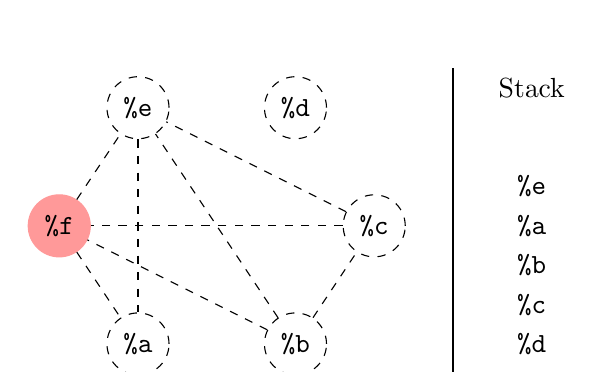
\begin{tikzpicture}
\node[circle, draw, dashed] (A) at (0,0)    {\tt \%a};
\node[circle, draw, dashed] (B) at (2,0)    {\tt \%b};
\node[circle, draw, dashed] (C) at (3,1.5)  {\tt \%c};
\node[circle, draw, dashed] (D) at (2,3)    {\tt \%d};
\node[circle, draw, dashed] (E) at (0,3)    {\tt \%e};
\node[circle, draw, fill, color=red!40] (F) at (-1,1.5) {\color{black}\tt \%f};

\draw[dashed] (B) -- (C);
\draw[dashed] (B) -- (E);
\draw[dashed] (B) -- (F);
\draw[dashed] (C) -- (E);
\draw[dashed] (C) -- (F);
\draw[dashed] (E) -- (A);
\draw[dashed] (F) -- (A);
\draw[dashed] (F) -- (E);

\node[] (S)  at (5,3.25) {Stack};
\node[] (S4) at (5,2)   {\tt \%e};
\node[] (S4) at (5,1.5) {\tt \%a};
\node[] (S3) at (5,1)   {\tt \%b};
\node[] (S2) at (5,.5)  {\tt \%c};
\node[] (S1) at (5,0)   {\tt \%d};

\draw (4, 3.5) -- (4, -.5);
\end{tikzpicture}
\end{center}

%%% 2
\begin{center}
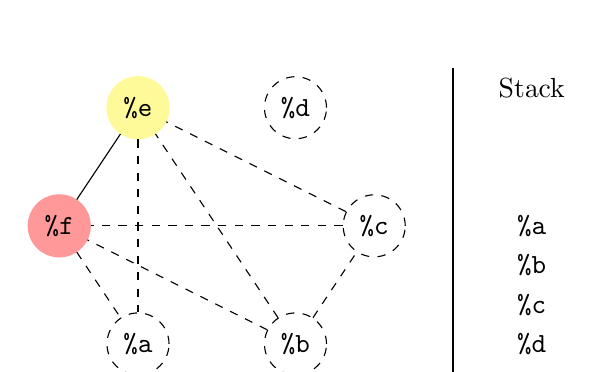
\begin{tikzpicture}
\node[circle, draw, dashed] (A) at (0,0)    {\tt \%a};
\node[circle, draw, dashed] (B) at (2,0)    {\tt \%b};
\node[circle, draw, dashed] (C) at (3,1.5)  {\tt \%c};
\node[circle, draw, dashed] (D) at (2,3)    {\tt \%d};
\node[circle, draw, fill, color=yellow!40] (E) at (0,3)    {\color{black}\tt \%e};
\node[circle, draw, fill, color=red!40] (F) at (-1,1.5) {\color{black}\tt \%f};

\draw[dashed] (B) -- (C);
\draw[dashed] (B) -- (E);
\draw[dashed] (B) -- (F);
\draw[dashed] (C) -- (E);
\draw[dashed] (C) -- (F);
\draw[dashed] (E) -- (A);
\draw[dashed] (F) -- (A);
\draw (F) -- (E);

\node[] (S)  at (5,3.25) {Stack};
\node[] (S4) at (5,1.5) {\tt \%a};
\node[] (S3) at (5,1)   {\tt \%b};
\node[] (S2) at (5,.5)  {\tt \%c};
\node[] (S1) at (5,0)   {\tt \%d};

\draw (4, 3.5) -- (4, -.5);
\end{tikzpicture}
\end{center}

%%% 3
\begin{center}
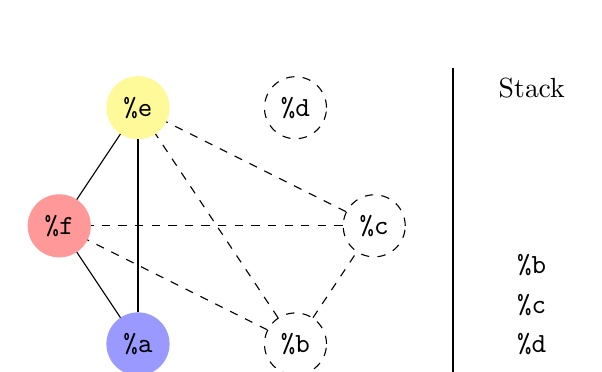
\begin{tikzpicture}
\node[circle, draw, fill, color=blue!40] (A) at (0,0)    {\color{black}\tt \%a};
\node[circle, draw, dashed] (B) at (2,0)    {\tt \%b};
\node[circle, draw, dashed] (C) at (3,1.5)  {\tt \%c};
\node[circle, draw, dashed] (D) at (2,3)    {\tt \%d};
\node[circle, draw, fill, color=yellow!40] (E) at (0,3)    {\color{black}\tt \%e};
\node[circle, draw, fill, color=red!40] (F) at (-1,1.5) {\color{black}\tt \%f};

\draw[dashed] (B) -- (C);
\draw[dashed] (B) -- (E);
\draw[dashed] (B) -- (F);
\draw[dashed] (C) -- (E);
\draw[dashed] (C) -- (F);
\draw (E) -- (A);
\draw (F) -- (A);
\draw (F) -- (E);

\node[] (S)  at (5,3.25) {Stack};
\node[] (S3) at (5,1)   {\tt \%b};
\node[] (S2) at (5,.5)  {\tt \%c};
\node[] (S1) at (5,0)   {\tt \%d};

\draw (4, 3.5) -- (4, -.5);
\end{tikzpicture}
\end{center}

%%% 4
\begin{center}
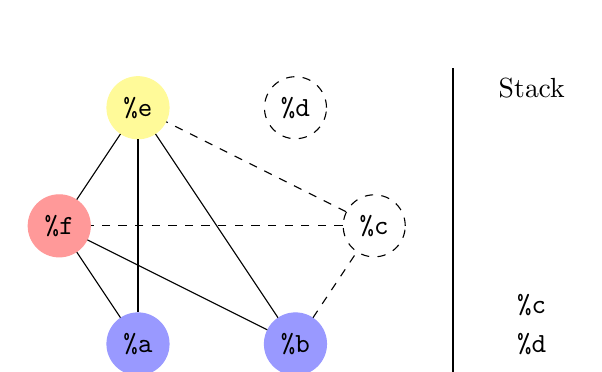
\begin{tikzpicture}
\node[circle, draw, fill, color=blue!40] (A) at (0,0)    {\color{black}\tt \%a};
\node[circle, draw, fill, color=blue!40] (B) at (2,0)    {\color{black}\tt \%b};
\node[circle, draw, dashed] (C) at (3,1.5)  {\tt \%c};
\node[circle, draw, dashed] (D) at (2,3)    {\tt \%d};
\node[circle, draw, fill, color=yellow!40] (E) at (0,3)    {\color{black}\tt \%e};
\node[circle, draw, fill, color=red!40] (F) at (-1,1.5) {\color{black}\tt \%f};

\draw[dashed] (B) -- (C);
\draw (B) -- (E);
\draw (B) -- (F);
\draw[dashed] (C) -- (E);
\draw[dashed] (C) -- (F);
\draw (E) -- (A);
\draw (F) -- (A);
\draw (F) -- (E);

\node[] (S)  at (5,3.25) {Stack};
\node[] (S2) at (5,.5)  {\tt \%c};
\node[] (S1) at (5,0)   {\tt \%d};

\draw (4, 3.5) -- (4, -.5);
\end{tikzpicture}
\end{center}

%%% 4
\begin{center}
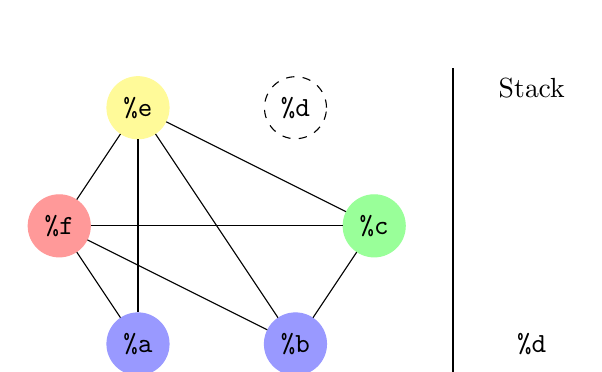
\begin{tikzpicture}
\node[circle, draw, fill, color=blue!40] (A) at (0,0)    {\color{black}\tt \%a};
\node[circle, draw, fill, color=blue!40] (B) at (2,0)    {\color{black}\tt \%b};
\node[circle, draw, fill, color=green!40] (C) at (3,1.5)  {\color{black}\tt \%c};
\node[circle, draw, dashed] (D) at (2,3)    {\tt \%d};
\node[circle, draw, fill, color=yellow!40] (E) at (0,3)    {\color{black}\tt \%e};
\node[circle, draw, fill, color=red!40] (F) at (-1,1.5) {\color{black}\tt \%f};

\draw (B) -- (C);
\draw (B) -- (E);
\draw (B) -- (F);
\draw (C) -- (E);
\draw (C) -- (F);
\draw (E) -- (A);
\draw (F) -- (A);
\draw (F) -- (E);

\node[] (S)  at (5,3.25) {Stack};
\node[] (S1) at (5,0)   {\tt \%d};

\draw (4, 3.5) -- (4, -.5);
\end{tikzpicture}
\end{center}

%%% 4
\begin{center}
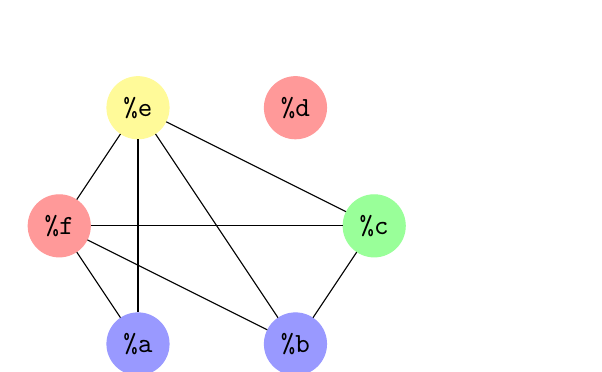
\begin{tikzpicture}
\node[circle, draw, fill, color=blue!40] (A) at (0,0)    {\color{black}\tt \%a};
\node[circle, draw, fill, color=blue!40] (B) at (2,0)    {\color{black}\tt \%b};
\node[circle, draw, fill, color=green!40] (C) at (3,1.5)  {\color{black}\tt \%c};
\node[circle, draw, fill, color=red!40] (D) at (2,3)    {\color{black}\tt \%d};
\node[circle, draw, fill, color=yellow!40] (E) at (0,3)    {\color{black}\tt \%e};
\node[circle, draw, fill, color=red!40] (F) at (-1,1.5) {\color{black}\tt \%f};

\draw (B) -- (C);
\draw (B) -- (E);
\draw (B) -- (F);
\draw (C) -- (E);
\draw (C) -- (F);
\draw (E) -- (A);
\draw (F) -- (A);
\draw (F) -- (E);

% Draw an invisible stack so everything lines up.
\node[] (S)  at (5,3.25) {\hphantom{Stack}};
\draw[color=white] (4, 3.5) -- (4, -.5);
\end{tikzpicture}
\end{center}

\noindent And this is what the final IR looks like:
\begin{Verbatim}
bb1:
    %r2 = ...
    %r1 = ...
    %r3 = add %r3, %r4
    branch on %r3 to bb2 else bb3
bb2:
    branch to bb4
bb3:
    %r2 = copy %r1
    branch to bb4
bb4:
    %r2 = phi [bb2: %r2], [bb3: %r1]
    %r1 = add %r3, %r2
\end{Verbatim}

\noindent If we emit this as x86\textunderscore64 ASM, the result might look a bit like this:
\begin{Verbatim}
.L1:
    ;; ...
    add rsi, rdx
    test rsi, rsi
    jnz .L2
    jmp .L3
.L2:
    jmp .L4
.L3:
    mov rdi, rax
    jmp .L4
.L4:
    mov rax, rsi
    add rax, rdi
\end{Verbatim}

\end{document}
